%Đây là template dùng cho đề cương đề tài tốt nghiệp
%Khoa Công nghệ Thông tin
%Trường Đại học Khoa học Tự nhiên, ĐHQG-HCM

%Liên hệ về mẫu LaTEX này: Thầy Bùi Huy Thông (bhthong@fit.hcmus.edu.vn)

\documentclass{article}[14pt]
\usepackage[utf8]{vietnam}
\usepackage{enumerate}
\usepackage{enumitem}
\usepackage{multicol}
\usepackage{listings}
\usepackage[left=2cm,right=2cm,top=2.5cm,bottom=2.5cm]{geometry}
\usepackage{verbatim}
\usepackage{graphicx}
\usepackage{url}
\usepackage{fancyhdr}
\usepackage{fancybox,framed}
\linespread{1.3}
\usepackage{lastpage}
\usepackage{floatrow}
\usepackage{floatrow}
\pagenumbering{arabic}
%\pagestyle{fancy}
\newfloatcommand{capbtabbox}{table}[][\FBwidth]

\usepackage{blindtext}
\usepackage{titlesec}
\usepackage[nottoc]{tocbibind}

\usepackage[table]{xcolor} % Để sử dụng \rowcolor và màu sắc trong bảng
\usepackage{float}          % Để sử dụng tùy chọn [H] giữ bảng đứng yên
\usepackage{array}          % Để hỗ trợ căn chỉnh cột tốt hơn

\titleformat*{\section}{\LARGE\bfseries}
\titleformat*{\subsection}{\Large\bfseries}
\titleformat*{\subsubsection}{\large\bfseries}
%\addbibresource{ref.bib}


\begin{document}
    \begin{figure}[h]
        \begin{floatrow}
        \ffigbox{
\includegraphics[scale = .4]{images/logo.png}}
        {%
    
        }
        \capbtabbox{
            \begin{tabular}{l}
            \multicolumn{1}{c}{\textbf{\begin{tabular}[c]{@{}c@{}}TRƯỜNG ĐẠI HỌC KHOA HỌC TỰ NHIÊN\\KHOA CÔNG NGHỆ THÔNG TIN\end{tabular}}} \\ \\ \\
            \end{tabular}
        }
        {%
    
        }
        \end{floatrow}
    \end{figure}
    
    \begin{center}
        
        %Xác định loại đề tài tốt nghiệp tương ứng: Khóa luận, Thực tập, Đồ án
        \textbf{\Large ĐỀ CƯƠNG KHOÁ LUẬN TỐT NGHIỆP} \\ 
    \end{center}
    
    %\vspace{.5cm}
    
    \begin{center}
    %Tên đề tài phải VIẾT HOA
        
        \textbf{\huge PHÁT TRIỂN HỆ THỐNG PHÂN ĐOẠN TỔN THƯƠNG XƯƠNG TRÊN ẢNH X-QUANG DỰA TRÊN CÂU NHẮC TRỰC QUAN}
        \\

    %Tên đề tài bằng tiếng Anh (nếu có)
    \vspace{.5cm}
        \textit{\textbf{\Large (Developing a bone lesion segmentation system on X-ray images based on visual prompts)}}
    \end{center}
    
    \vspace{.5cm}
    
    \Large
    \section{THÔNG TIN CHUNG}
    \begin{itemize}[label = {}]
        
        \item \textbf{Người hướng dẫn:} 
        %Thể hiện dạng: <Chức danh> <Họ và tên> (<Đơn vị công tác>)
        \begin{itemize}
            \item PGS.TS. Lý Quốc Ngọc (Khoa Công nghệ Thông tin)
            \item ThS. Đỗ Thị Thanh Hà (Khoa Công nghệ Thông tin)
        \end{itemize}{}
    
        
        \item \textbf{Nhóm sinh viên thực hiện:}
        
        %Thể hiện dạng: <Họ và tên sinh viên> (MSSV: )
        \begin{enumerate}
        
            \item Nguyễn Hữu Bình (MSSV: 22120031) 
            \item Thông Lúc (MSSV: 22120196)
        \end{enumerate}

       %Chọn loại thích hợp
        \item \textbf{Loại đề tài:} Nghiên cứu
        
        \item \textbf{Thời gian thực hiện:} Từ \textit{01/2026} đến \textit{07/2026}
        
    \end{itemize}
    
    \pagebreak 
    
    \section{NỘI DUNG THỰC HIỆN}
    {

    \subsection{Giới thiệu về đề tài}
    
    Chẩn đoán hình ảnh thông qua X-quang đóng vai trò then chốt trong việc phát hiện các tổn thương xương như gãy xương, thoái hóa hay các khối u. Tuy nhiên, việc phân đoạn thủ công các vùng tổn thương này tốn rất nhiều thời gian và phụ thuộc lớn vào kinh nghiệm của bác sĩ. Mặc dù các mô hình học sâu tự động như U-Net đã đạt được nhiều thành công, chúng vẫn gặp khó khăn trong việc xử lý các ca bệnh phức tạp nơi ranh giới giữa mô lành và tổn thương không rõ ràng.
    
    Đề tài đề xuất phát triển một hệ thống phân đoạn ảnh X-quang xương tương tác dựa trên cơ chế \textit{câu nhắc trực quan} (visual prompts). Thay vì để mô hình tự suy luận mù quáng, hệ thống cho phép bác sĩ định hướng vùng quan tâm thông qua một hộp giới hạn sơ bộ. Điểm cốt lõi của đề tài là kiến trúc \textbf{PGA-UNet} (Prompt-Guided Attention U-Net), tích hợp sâu thông tin câu nhắc vào cả quá trình mã hóa và giải mã để tối ưu hóa sự tập trung của mô hình. Ngoài ra, hệ thống còn được thiết kế với cơ chế phòng vệ tự động để đảm bảo tính an toàn y tế ngay cả khi bác sĩ cung cấp câu nhắc không chính xác.

    \subsection{Mục tiêu đề tài}
    
    Mục tiêu chính của đề tài là xây dựng một hệ thống hỗ trợ chẩn đoán hình ảnh toàn diện, giúp bác sĩ bóc tách nhanh chóng và chính xác các cấu trúc xương tổn thương. Cụ thể:
    \begin{itemize}
        \item Nghiên cứu và triển khai kiến trúc \textbf{PGA-UNet} với hai thành phần cải tiến: Cổng không gian (Prompt Spatial Gate) ở Encoder và Cơ chế chú ý có điều kiện (Conditioned Attention) ở Decoder.
        \item Đạt được hiệu năng phân đoạn vượt trội so với các mô hình tự động truyền thống, với chỉ số Dice dự kiến trên 85\%.
    \end{itemize}
    
    \subsection{Phạm vi của đề tài}
    
    Nghiên cứu tập trung vào bài toán phân đoạn ảnh X-quang xương 2D, đặc biệt là các vùng xương có cấu trúc phức tạp như cổ chân, gót chân. Hệ thống được thiết kế để xử lý các ảnh có độ tương phản thấp và chứa nhiều nhiễu kỹ thuật. Phạm vi thực nghiệm bao gồm việc huấn luyện và đánh giá trên bộ dữ liệu X-quang đã được chuyên gia gán nhãn mức điểm ảnh. Đề tài không mở rộng sang dữ liệu 3D (CT/MRI) mà tập trung tối ưu hóa trải nghiệm tương tác và độ tin cậy của mô hình trên mặt phẳng 2D trong điều kiện thực tế lâm sàng.
 
    \subsection{Cách tiếp cận thực hiện}
    
    Hệ thống được thiết kế theo luồng xử lý đầu-cuối (end-to-end pipeline) gồm hai giai đoạn:
    
    \textbf{1. Giai đoạn huấn luyện (Offline):} 
    Thực hiện tiền xử lý ảnh (loại bỏ ký tự nhiễu, cân bằng histogram). Huấn luyện mô hình phân lớp bệnh lý để sàng lọc ban đầu và mô hình PGA-UNet để phân đoạn. Câu nhắc trong giai đoạn này được sinh tự động từ nhãn gốc dưới dạng bản đồ nhiệt Gaussian (Gaussian Heatmap).
    
    \textbf{2. Giai đoạn suy luận tương tác (Online):} 
    Tích hợp các mô hình vào giao diện phần mềm. Khi bác sĩ khoanh vùng (Bounding Box), hệ thống chuyển đổi thành câu nhắc trực quan để kích hoạt PGA-UNet và trả về mặt nạ phân đoạn.

    \vspace{.5cm}
    \begin{figure}[H]
        \centering
        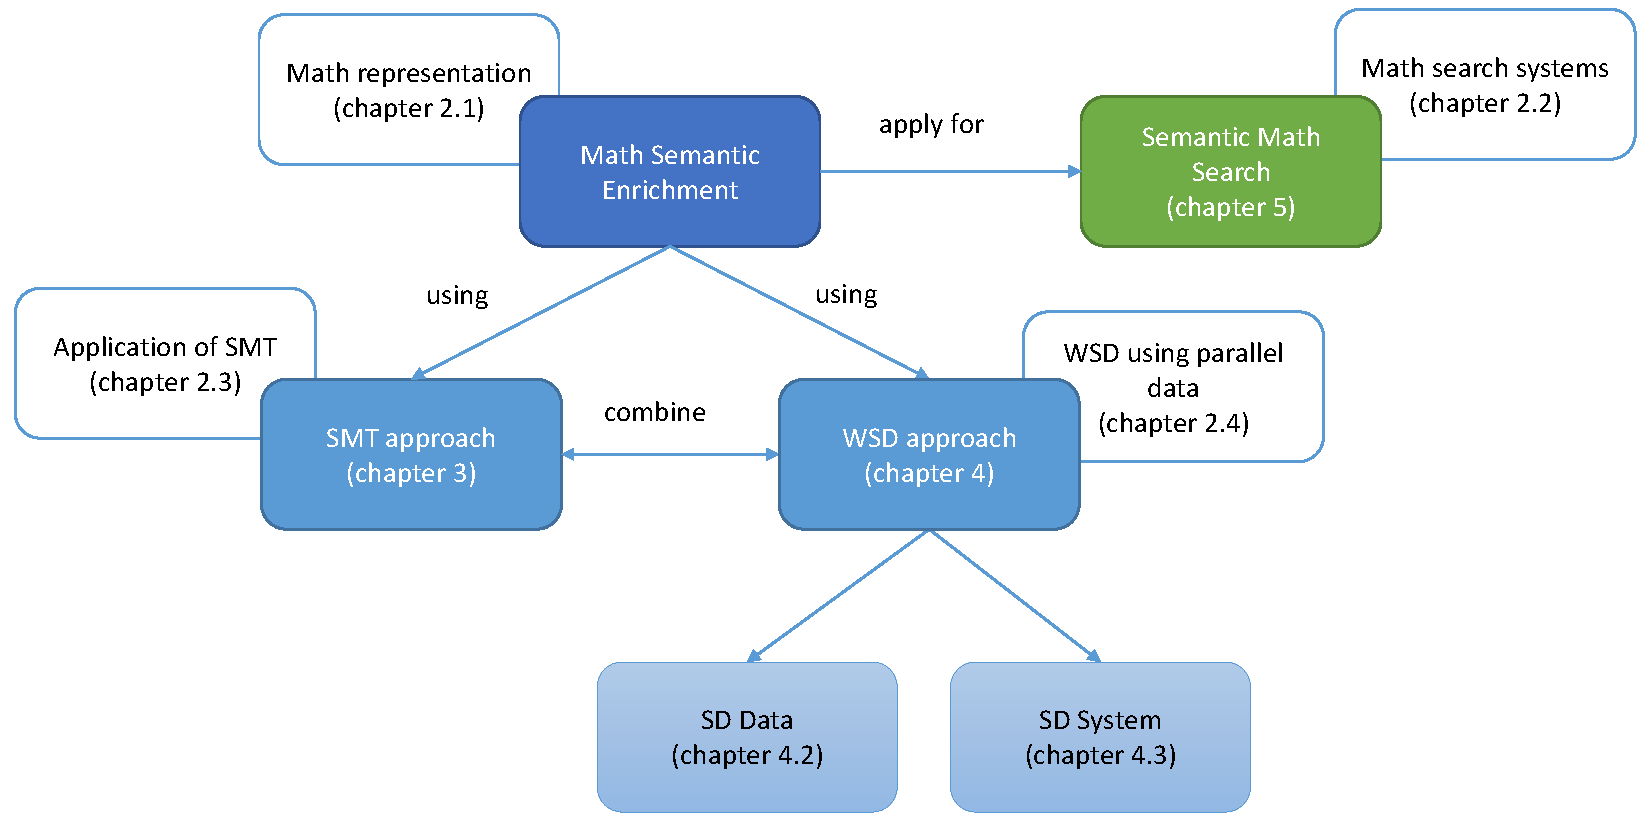
\includegraphics[width=0.9\textwidth]{images/Overview.pdf}
        \caption{Sơ đồ kiến trúc tổng thể của hệ thống đề xuất (PGA-UNet Pipeline)}
        \label{fig:sodo_pga}
    \end{figure}
    \vspace{.5cm}
    
    Sự kết hợp giữa tri thức hình học (Gaussian Heatmap) và đặc trưng ngữ nghĩa (Deep Features) thông qua cơ chế Attention giúp mô hình có khả năng hội tụ cực nhanh và đạt độ chính xác cao ngay cả với tập dữ liệu huấn luyện nhỏ.
    
    \subsection{Kết quả dự kiến của đề tài}
        
    Sản phẩm của đề tài bao gồm một hệ thống hoàn chỉnh với các kết quả định lượng và định tính như sau:
    \begin{itemize}
        \item \textbf{Định lượng:} Mô hình PGA-UNet đạt Dice = 0.8524 (kịch bản Zoom-out) và Dice = 0.8382 (kịch bản Shift), vượt xa U-Net (0.4534) và SAM-Med2D fine-tuned (0.7350) trên tập kiểm thử 232~mẫu per-polygon.
        \item \textbf{Định tính:} Tính bền bỉ (robustness) tốt trước các sai số của người dùng. Tốc độ suy luận đạt mức thời gian thực (< 1 giây/ảnh).
        \item \textbf{Sản phẩm:} Bộ mã nguồn huấn luyện/suy luận ổn định, bộ trọng số mô hình đã tối ưu, và ứng dụng Demo cho phép bác sĩ tương tác trực tiếp bằng câu nhắc.
    \end{itemize}

    \subsection{Kế hoạch thực hiện}
    
    Kế hoạch thực hiện được chi tiết hóa theo các mốc thời gian để đảm bảo tiến độ hoàn thành khóa luận:

    \begin{table}[H]
    \centering
    \renewcommand{\arraystretch}{1.5}
    \begin{tabular}{|p{3.5cm}|p{7.5cm}|p{5cm}|}
    \hline
    \rowcolor[gray]{0.9} \textbf{Mốc thời gian} & \textbf{Nội dung công việc} & \textbf{Phân công thực hiện} \\ \hline
    
    01/01 - 25/01/2026 & Tìm hiểu cơ chế Attention, Visual Prompts và các kỹ thuật tiền xử lý ảnh X-quang. & Nguyễn Hữu Bình, Thông Lúc \\ \hline
    
    26/01 - 05/02/2026 & Thu thập và tiền xử lý dữ liệu, gán nhãn và làm sạch nhiễu ký tự. & Nguyễn Hữu Bình, Thông Lúc\\ \hline
    
    06/02 - 28/02/2026 & Thiết kế kiến trúc PGA-UNet và cơ chế Prompt Spatial Gate. & Nguyễn Hữu Bình, Thông Lúc \\ \hline
    
    01/03 - 11/03/2026 & Xây dựng Đề cương khóa luận chi tiết và thiết lập môi trường PyTorch. & Nguyễn Hữu Bình, Thông Lúc \\ \hline
    
    12/03 - 22/03/2026 & Huấn luyện mô hình phân lớp sàng lọc và PGA-UNet cơ bản. & Nguyễn Hữu Bình, Thông Lúc \\ \hline
    
    23/03 - 30/04/2026 & Thực nghiệm và đánh giá tính bền bỉ (robustness) của hệ thống. & Nguyễn Hữu Bình, Thông Lúc \\ \hline

    01/05 - 20/05/2026 & Tinh chỉnh siêu tham số, huấn luyện với hàm mất mát kết hợp BCE-Dice. & Nguyễn Hữu Bình, Thông Lúc \\ \hline
    
    21/05 - 05/06/2026 & Đánh giá hiệu năng trên tập test, so sánh với Baseline U-Net. & Nguyễn Hữu Bình, Thông Lúc \\ \hline
    
    06/06 - 15/06/2026 & Hoàn thiện báo cáo khóa luận (LaTeX) và đóng gói mã nguồn. & Nguyễn Hữu Bình, Thông Lúc \\ \hline
    
    16/06 - 20/06/2026 & Xây dựng ứng dụng Demo và chuẩn bị Slide bảo vệ. & Nguyễn Hữu Bình, Thông Lúc \\ \hline
    
    07/2026 & Chỉnh sửa theo góp ý của GVHD và Bảo vệ khóa luận. & Nguyễn Hữu Bình, Thông Lúc \\ \hline
    
    \end{tabular}
    \caption{Bảng kế hoạch thực hiện chi tiết}
    \end{table}
    }
    \pagebreak 
    %TÀI LIỆU TRÍCH DẪN
    \bibliographystyle{ieeetr}
    \bibliography{sample}
    \nocite{*}

    \begin{table}[h]
    \centering
        \begin{tabular{p{7cm}p{7cm}}
        \textbf{\begin{tabular}[c]{@{}c@{}}\\XÁC NHẬN\\CỦA NGƯỜI HƯỚNG DẪN\\ \textit{(Ký và ghi rõ họ tên)}\end{tabular}} & \textbf{\begin{tabular}[c]{@{}c@{}}\textit{TP. Hồ Chí Minh, ngày... tháng... năm...}\\NHÓM SINH VIÊN THỰC HIỆN\\\textit{(Ký và ghi rõ họ tên}) \end{tabular}}
        \end{tabular}
    \end{table}
    
\end{document}
